% IEEE ISBI 2027 four-page paper (official spconf template). The whole paper,
% including references, fits in four pages: no paid fifth page.
\documentclass{article}
\usepackage{spconf,amsmath,amssymb,graphicx,booktabs,array,url,microtype,balance}
\usepackage[hidelinks]{hyperref}
\usepackage{xcolor}

% Values still to be filled from reports/isbi_submission_latest (workstation).
% Every \pend must be gone before submission; the build log lists survivors.
\newcommand{\pend}[1]{\textcolor{red}{#1}\typeout{PENDING VALUE: #1}}
% Wording that depends on which way a pending result falls; both branches are
% drafted in SUBMISSION_CHECKLIST.md. Remove the wrapper once confirmed.
\newcommand{\decide}[1]{\textcolor{red}{#1}\typeout{DECIDE BRANCH: #1}}
% Workstation numbers: scripts/build_isbi_numbers.py writes numbers.tex.
\InputIfFileExists{numbers.tex}{}{}
\providecommand{\numXfInlAUROC}{\pend{.00}}
\providecommand{\numSpInlAUROC}{\pend{.00}}
\providecommand{\numXfPerspAUROC}{\pend{.00}}
\providecommand{\numSpPerspAUROC}{\pend{.00}}
\providecommand{\numXfComboAUROC}{\pend{.00}}
\providecommand{\numSpComboAUROC}{\pend{.00}}
\providecommand{\numSrComboAUROC}{\pend{.00}}
\providecommand{\numInlAUROCRange}{\pend{0.XX}}
\providecommand{\numNestedPrecision}{\pend{XX\%}}
\providecommand{\numNestedTau}{\pend{X.X}}
\providecommand{\numNestedRecall}{\pend{XX\%}}
\providecommand{\numCondDelta}{\pend{+0.00X}}
\providecommand{\numLogRevXf}{\pend{0/0}}
\providecommand{\numLogRevSp}{\pend{0/0}}
\providecommand{\numLogAucB}{\pend{.000}}
\providecommand{\numLogAucS}{\pend{.000}}
\providecommand{\numLogRevTotal}{\pend{N}}
\providecommand{\numQuantRevXf}{\pend{0/0}}
\providecommand{\numQuantRevSp}{\pend{0/0}}
\providecommand{\numQuantAucB}{\pend{.000}}
\providecommand{\numQuantAucS}{\pend{.000}}
\providecommand{\numQuantRevTotal}{\pend{N}}
\providecommand{\numSampledMisses}{\pend{N}}
\providecommand{\numSampledMissesSift}{\pend{0/0}}
\providecommand{\numInverseOnly}{\pend{N}}
\providecommand{\numInverseOnlyFailed}{\pend{N}}
\providecommand{\numReflections}{\pend{N}}
\providecommand{\numQuadPasses}{\pend{N}}
\providecommand{\numRansacXf}{\pend{0/0/0}}
\providecommand{\numRansacSp}{\pend{0/0/0}}
\providecommand{\numRansacSift}{\pend{0/0/0}}
\providecommand{\numRansacSr}{\pend{0/0/0}}
\providecommand{\numMoisanLeft}{\pend{Z}}
\providecommand{\numPoleRescued}{\pend{X}}
\providecommand{\numPoleExplicit}{\pend{Y}}
\providecommand{\numPoleSilent}{\pend{Y}}
\providecommand{\numSiftToSilent}{\pend{N}}
\providecommand{\numChangedNonPole}{\pend{N}}
\providecommand{\numNetSuccess}{\pend{$\pm$0}}
\providecommand{\numSrReturned}{\pend{000}}
\providecommand{\numSrFailed}{\pend{000}}
\providecommand{\numSrRect}{\pend{0/0}}
\providecommand{\numSrFov}{\pend{0/0}}
\providecommand{\numSrRho}{\pend{0/0}}
\providecommand{\numSrRectCount}{\pend{N}}
\providecommand{\numSrZeroInlier}{\pend{N}}
\providecommand{\numSrPoleGroups}{\pend{N}}
\providecommand{\numSrRefitPoles}{\pend{N}}
\providecommand{\numSrClrAUROC}{\pend{.000}}
\providecommand{\numSrInlAUROC}{\pend{.00}}
\providecommand{\numSrPerspAUROC}{\pend{.00}}
\providecommand{\numSrFireDiff}{\pend{0.0XX}}
\providecommand{\numXfClrCI}{\pend{?}}
\providecommand{\numSpClrCI}{\pend{?}}
\providecommand{\numSrClrCI}{\pend{?}}
\providecommand{\numXfInlCI}{\pend{?}}
\providecommand{\numSpInlCI}{\pend{?}}
\providecommand{\numSrInlCI}{\pend{?}}
\providecommand{\numXfFusedCI}{\pend{?}}
\providecommand{\numSpFusedCI}{\pend{?}}
\providecommand{\numSrFusedCI}{\pend{?}}
\providecommand{\numSpFusedInlDiff}{\pend{?}}
\providecommand{\numSrFusedInlDiff}{\pend{?}}
\providecommand{\numXfFusedInlDiff}{\pend{?}}
\providecommand{\numXfFusedDetDiff}{\pend{?}}
\providecommand{\numSpFusedDetDiff}{\pend{?}}
\providecommand{\numSrWithInl}{\pend{?}}
\providecommand{\numSrWithInlClr}{\pend{?}}
\providecommand{\numSrWithInlInl}{\pend{?}}
\providecommand{\numClrPerspBound}{\pend{?}}
\providecommand{\numSensSp}{\pend{?}}
\providecommand{\numSensSr}{\pend{?}}
\providecommand{\numSensXf}{\pend{?}}
\providecommand{\numCrossFailLoose}{\pend{?}}
\providecommand{\numReturnedShift}{\pend{?}}
\providecommand{\numSensMinFused}{\pend{?}}
\providecommand{\numSensMinClr}{\pend{?}}
\providecommand{\numSensMinInl}{\pend{?}}

\title{SILENT FOLDS: PROJECTIVE POLES AS A TRAINING-FREE FAILURE FLAG\\
IN HOMOGRAPHY-BASED RETINAL REGISTRATION}
\name{Felix Bergmann}
\address{University of Amsterdam, Amsterdam, The Netherlands\\
\texttt{felix.bergmann2@student.uva.nl}}

\newcommand{\xf}{XFeat-H}
\newcommand{\splg}{SPLG-H}
\newcommand{\sift}{SIFT-H}
\newcommand{\sr}{SuperRetina}
\newcommand{\ci}[1]{\,{\scriptsize(#1)}}

\begin{document}
\ninept
\maketitle

\begin{abstract}
Homographies remain the default transform in feature-based retinal
registration, yet every homography has a pole line on which its denominator
vanishes. Where that line crosses the fundus the warp folds, while the matrix
still looks valid. Auditing 625 FIRE and COph100 pairs registered with XFeat,
SuperPoint/LightGlue, and the released retina-specific SuperRetina, we find
that all 100 image crossings are failures, 25 of them not flagged by the
estimator, and 167 of the 168 estimates within one image diagonal of a pole
fail; every crossing still fails at twice the error threshold. The pole
clearance $\rho$, a unit-free distance from a few denominator evaluations, is
a training-free quality-control (QC) score (area under the ROC curve, AUROC,
0.78--0.85 at the study endpoint). Fused with RANSAC inlier ratio it reaches 0.85--0.86,
significantly above inlier ratio for two of three pipelines and not
significantly different from a learned detector, and it stays at or above
0.75 across endpoints from 0.0025 to 0.02 of the image diagonal, where
either score alone drops to 0.47--0.56 on some pipeline. The rectangle crossing test is equivalent to the common
projected-corner check; we extend it to circular and convex supports. Poles
also corrupt learned QC: two pole estimates were involved in 19 of 20
Platt-calibration reversals of a detector across 21 regroupings. A guard on the feature's own
support removes all of them and lowers the worst-case Brier score; a guard on
a narrower support removes none.
\end{abstract}

\begin{keywords}
retinal image registration, quality control, homography, failure detection, calibration
\end{keywords}

\section{Introduction}
\label{sec:intro}

Registration of fundus photographs underlies longitudinal monitoring and
screening, for example of retinopathy of prematurity in infants
\cite{coph,ridirp}. A silently failed registration corrupts every downstream
change measurement, so at scale failures must be caught automatically.
Feature-based retinal methods still estimate a homography: SuperRetina fits
one to learned keypoints \cite{superretina}, and SuperJunction uses one as its
first stage \cite{superjunction}. Registration quality control (QC), in turn, predicts failure
from appearance, match, and transformation features such as Jacobians and
bending energy \cite{bierbrier,sokooti,octfundusreg}.

\begin{figure*}[t]
\centering
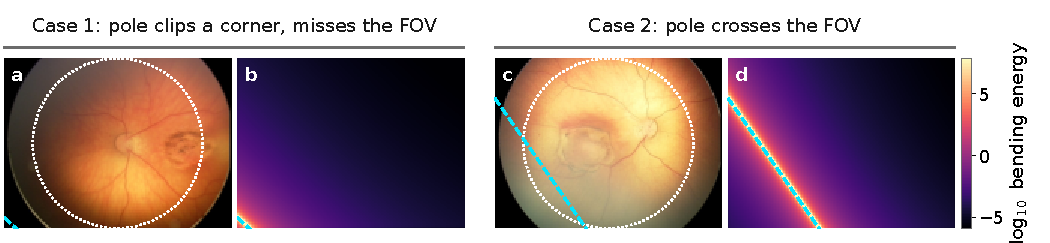
\includegraphics[width=\textwidth]{assets/qualitative_pole.pdf}
\vspace{-6mm}
\caption{Two failed COph100 \xf{} registrations (patient 055). (a,c) Moving
fundus images; (b,d) log bending-energy density of the estimated warp on one
shared scale. Cyan: pole line $d=0$; dotted: inscribed-FOV proxy. In case 1
the pole clips the rectangle but misses the FOV and the fundus mask; in case 2
it crosses the FOV along a 294.9-pixel chord. Images: RIDIRP (CC0);
annotations: COph100 (CC BY 4.0) \cite{ridirp,coph}.}
\label{fig:poles}
\end{figure*}

\begin{table*}[t]
\centering\small
\caption{Pole audit on 625 retinal pairs. Failed / flagged: returned transforms that fail among
those each criterion flags. AUROCs are pooled and group-weighted over all attempted
pairs, with 95\% group-bootstrap intervals; inlier ratio is a pre-specified
training-free baseline (for \sr{}, its LMedS inlier rate); fused: mean rank
percentile of ${-}\log\rho$ and inlier ratio; detector: median raw AUROC of
the guarded Base detector over 21 assignments. Constrained RANSAC
(rectangle): failures made successes / silent failures made explicit /
explicit failures made silent; for \sr{}, the study RANSAC re-fits its
stage-1 matches. \sift{} is a weak-matching stress test.}
\label{tab:audit}
\setlength{\tabcolsep}{3pt}
\begin{tabular}{lrrrrrllllr}
\toprule
 & & & \multicolumn{3}{c}{Failed / flagged} & \multicolumn{4}{c}{AUROC} & Constr. \\
\cmidrule(lr){4-6}\cmidrule(lr){7-10}
Pipeline & Returned & Failed & Rect.\ cross. & FOV cross. & $\rho\le1$ & ${-}\log\rho$ & Inlier ratio & Fused & Detector & RANSAC \\
\midrule
\xf{}   & 625 & 342 & 2/2   & 1/1   & 20/21 & .778\ci{\numXfClrCI} & \numXfInlAUROC\ci{\numXfInlCI} & \numXfComboAUROC\ci{\numXfFusedCI} & .833 & \numRansacXf \\
\splg{} & 618 & 278 & 10/10 & 6/6   & 40/40 & .823\ci{\numSpClrCI} & \numSpInlAUROC\ci{\numSpInlCI} & \numSpComboAUROC\ci{\numSpFusedCI} & .838 & \numRansacSp \\
\sr{}   & \numSrReturned & \numSrFailed & \numSrRect & \numSrFov & \numSrRho & \numSrClrAUROC\ci{\numSrClrCI} & \numSrInlAUROC\ci{\numSrInlCI} & \numSrComboAUROC\ci{\numSrFusedCI} & -- & \numRansacSr \\
\midrule
\sift{} & 521 & 519 & 375/375 & 187/187 & 412/412 & -- & -- & -- & -- & \numRansacSift \\
\bottomrule
\end{tabular}
\vspace{-2mm}
\end{table*}

A homography is a rational map. Where its projective denominator changes sign
it sends image points through infinity and reverses orientation, a
\emph{fold}: in a fundus overlay, the moving image is torn along the pole line
and the part beyond it is mirrored onto the far side. Close to that line its
derivatives are unbounded. Robust estimators do not test for this: RANSAC
scores reprojection consensus, and the returned matrix is finite. Moisan et
al.\ reject such ``wild homographies'' by enforcing orientation preservation
at the four sample points \cite{moisan}, which constrains those points but
not the rest of the image.

\textbf{Contributions.} (1) An audit of three modern retinal pipelines on
FIRE and COph100 \cite{fire,coph}, including the released \sr{}: pole
crossings are always failures, often silent ones, and pole distance is a
training-free QC score that adds to inlier ratio. (2) Tools: the rectangle
crossing test is algebraically the common projected-corner convexity check;
we extend it to circular and convex supports, normalize the pole distance
into a scale-invariant clearance, and apply it as a RANSAC hypothesis
constraint. (3) A cautionary finding for learned QC: homography-derived
derivative features are unbounded, so a detector must guard, transform, or
drop them, and a guard must contain the feature's support.

\section{Method}
\label{sec:method}

\textbf{Pole and folding.} A homography $H$ maps $(x,y)$ to
\begin{equation}
u=\frac{h_{11}x+h_{12}y+h_{13}}{d},\quad
v=\frac{h_{21}x+h_{22}y+h_{23}}{d},
\label{eq:h}
\end{equation}
with denominator $d(x,y)=h_{31}x+h_{32}y+h_{33}$ and Jacobian determinant
$\det J(x,y)=\det H/d(x,y)^3$ \cite{hartley}. Hence $\det J$ changes sign
exactly where $d$ does: the pole line $d=0$ is the fold, and $|\det J|$, like
every higher derivative, diverges as $d\to0$.

\textbf{Exact support tests.} Because $d$ is affine, its extrema on an
axis-aligned rectangle lie at the four corners $c_k$, so the pole crosses the
closed rectangle if and only if
\begin{equation}
\min_k d(c_k)\le0\le\max_k d(c_k).
\label{eq:corner}
\end{equation}
This is the algebraic form of the common check that the projected corners
form a convex quadrilateral with the source orientation: a corner triangle's
image orientation is $\mathrm{sign}(\det H)\,\mathrm{sign}(d_id_jd_k)$, so
the two agree unless a corner lies on the pole. Unlike the projected check,
Eq.~(\ref{eq:corner}) extends to any convex support, such as a fundus mask's
convex hull, by evaluating $d$ at its vertices (for a non-convex mask this is
conservative). For a circular field of view (FOV) with center $q$ and radius $r$, with
$a=(h_{31},h_{32})$, the condition is $|a^\top q+h_{33}|\le r\lVert
a\rVert_2$; we use the image's inscribed circle as the FOV proxy. $H$ maps
moving to fixed image and is tested on the moving support; $H^{-1}$ is tested
on the fixed image.

\textbf{Clearance.} For a non-crossing rectangle with diagonal $L$,
\begin{equation}
\rho(H)=\min_k|d(c_k)|\,/\,\bigl(L\lVert a\rVert_2\bigr)
\label{eq:clearance}
\end{equation}
is the distance from the image to the pole line in image diagonals; $\rho=0$
for a crossing and $\rho=\infty$ for an affine map. It is invariant to matrix
scale and image resolution and costs four denominator evaluations.

\textbf{Uses.} (i) \emph{QC score}: $s=-\log_{10}\max(\rho,10^{-3})$, with
$\rho$ capped at $10^{3}$; the \emph{fused} score averages the rank
percentiles of $s$ and of the negated RANSAC inlier ratio. Neither is
trained. (ii) \emph{Feature guard}: a derivative feature is set missing when
the pole crosses the support on which it is computed. (iii)
\emph{Support-constrained RANSAC}: minimal-sample hypotheses whose pole
crosses the support are discarded before consensus scoring, on the same
random stream; if the consensus refit crosses, the best admissible hypothesis
is returned, and if none exists the registration fails explicitly.

\section{Experimental setup}
\label{sec:setup}

\textbf{Data and endpoint.} We use 134 FIRE \cite{fire} and 491 COph100
\cite{coph} pairs, grouped into 42 image-connected FIRE components (patient
identifiers are unavailable) and 56 COph100 patients. A registration fails if
it returns no transform (an \emph{explicit} failure) or its mean landmark
error exceeds 0.005 of the fixed-image diagonal in original coordinates (a
\emph{silent} failure): 20.6 pixels on FIRE ($2912^2$), within its standard
0--25-pixel success curve, and 4 pixels on COph100 ($640\times480$).

\textbf{Pipelines.} The generic (not retina-specific) pipelines \xf{},
\splg{}, and \sift{} match XFeat \cite{xfeat},
SuperPoint/LightGlue \cite{lightglue}, or SIFT \cite{sift} correspondences at
a 1,024-pixel long edge (COph100 upsampled $1.6\times$) and share one seeded
RANSAC with a normalized DLT (3-px threshold, $10^4$ iterations, consensus
refit). \sr{} is run as released (least-median-of-squares, LMedS, with its two-pass
refinement) at
original resolution \cite{superretina}; it reproduces the published FIRE
success-curve AUCs of the S/P/A (large-overlap/small-overlap/anatomical-change)
categories within \numSrFireDiff.

\textbf{Learned detector.} Per pipeline, an L2-regularized logistic
regression combines image, match, inverse-consistency, geometric (including
bending energy $\mathcal{B}$ on a $32\times32$ lattice, our curvature
feature), cross-pipeline, and structure features (Base); a second arm adds
resampling and perturbation stability (+Stab). Features are standardized
after training-median imputation with one missingness indicator each, and
$C\in\{0.1,1,10\}$ is chosen by grouped inner cross-validation. Platt scaling
\cite{platt}, an unregularized logistic fit of the raw score, uses a disjoint
calibration fold; a negative slope reverses the ranking. With five group
folds (test $f$, calibration $f{+}1$, training the rest), we refit everything
under 21 seeded group-to-fold assignments and pool test predictions with
equal total weight per patient group. Assignment spread reuses cases and is
not a confidence interval; intervals are 95\% group bootstraps (2,000
resamples of patients or components) on the original assignment. No-output
pairs receive the most-failing value of every training-free score.

\section{Results}
\label{sec:results}

\begin{figure}[t]
\centering
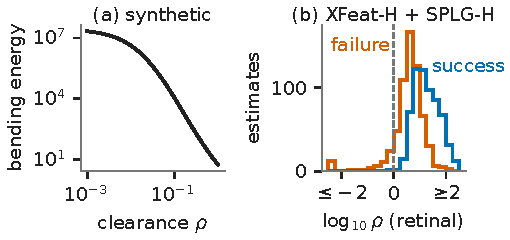
\includegraphics[width=\columnwidth]{assets/clearance_qc.pdf}
\vspace{-6mm}
\caption{(a) Bending energy on the $32\times32$ lattice for a synthetic
homography whose pole approaches a $640\times480$ image from outside.
(b) Clearance of all returned \xf{} and \splg{} estimates; $\le\!-2$ holds the
12 crossings. Dashed: $\rho=1$, left of which 60/61 estimates fail.}
\label{fig:clearance}
\vspace{-3mm}
\end{figure}

\subsection{Pole crossings are failures, often silent}

All 12 crossings by the generic matchers are failures
(Table~\ref{tab:audit}); they come from four COph100 patients and none from
FIRE. \sr{} with its own LMedS returns \numSrRectCount{} crossing
homographies from \numSrPoleGroups{} COph100 patients, all failures;
\numSrZeroInlier{} have no LMedS inliers, which its evaluation counts as
failed, but 13 would pass silently. Testing $H^{-1}$ on the fixed image adds
\numInverseOnly{} \splg{} crossings (\numInverseOnlyFailed{} failed); none of
the estimates is a global reflection. The projected-corner check flags the
same crossings, as it must; the $32\times32$ lattice $\det J$ test costs 256
times more and misses \numSampledMissesSift{} \sift{} crossings. Under weak
matching, invalid geometry is common: 72\% of \sift{} homographies cross the
image. Crossings alone have low recall (12 of 620 generic-matcher failures);
the clearance extends them: within one diagonal, 60 of 61 generic-matcher and
all 107 \sr{} estimates fail (Fig.~\ref{fig:clearance}b). This does not
depend on the endpoint: all crossings fail up to 0.01 of the diagonal and
\numCrossFailLoose{} at 0.02, and restricting to returned transforms changes
no AUROC below by more than \numReturnedShift.

\subsection{Clearance is a training-free QC score}

${-}\log\rho$ reaches AUROC 0.778/0.823/0\numSrClrAUROC{} for
\xf{}/\splg{}/\sr{} (Table~\ref{tab:audit}). Inlier ratio is stronger on
\xf{} (0\numXfInlAUROC) and weaker on the others
(0\numSpInlAUROC/0\numSrInlAUROC). The two are complementary: the fused score
exceeds inlier ratio on \splg{} and \sr{} (paired 95\% intervals of the
AUROC difference \numSpFusedInlDiff{} and \numSrFusedInlDiff) but not on
\xf{} (\numXfFusedInlDiff), and is not significantly different from the
learned detector (\numXfFusedDetDiff, \numSpFusedDetDiff). On \sr{}
estimates with at least one inlier (\numSrWithInl), $\rho$ still reaches
\numSrWithInlClr{} versus \numSrWithInlInl. The pole distance from the image
center ranks identically (differences within $\pm$\numClrPerspBound): the
exact support matters for the crossing decision and the unit threshold, not
for ranking. A warped-area scale baseline reaches only 0.68/0.70 (\xf{}/\splg{}). Flagging
$\rho\le\tau$ with $\tau$ chosen on training groups for $\ge$95\% precision
keeps \numNestedPrecision{} held-out precision at \numNestedRecall{} recall
(median $\tau=\numNestedTau$ diagonals). At looser endpoints (0.01/0.02 of
the diagonal), the AUROC of $\rho$ rises for \splg{} and \sr{}
(\numSensSp, \numSensSr) but falls for \xf{} (\numSensXf), whose near-pole
estimates are often only moderately wrong, while inlier ratio degrades on
\splg{}. The fused score is the robust choice: across endpoints from 0.0025
to 0.02 its lowest AUROC is \numSensMinFused{}, versus \numSensMinClr{} for
$\rho$ and \numSensMinInl{} for inlier ratio.

\subsection{Poles corrupt learned calibration}

In one held-out fold (\xf{}, +Stab, original assignment), the raw detector ranks failures well
(AUROC 0.927), but its Platt slope is $-4.3\times10^{-5}$, compressing all 83
test probabilities into $[0.57961,0.57970]$ and reversing them (0.073). The
calibration fold held the two patient-055 poles of Fig.~\ref{fig:poles},
whose bending energies ($8.65\times10^{9}$, $1.05\times10^{9}$) lie orders of
magnitude outside the training range; deleting both restores the fit,
deleting either alone does not. The 20 reversals across 21 assignments
repeat this mechanism rather than adding independent evidence: 19 reuse
these two estimates, and one \splg{} fold holds six poles from two patients.
The cause is geometric: moving a synthetic pole from $\rho=1$ to $10^{-3}$
outside a $640\times480$ image raises lattice bending energy from 5.53 to
$2.13\times10^{7}$ (Fig.~\ref{fig:clearance}a).

\begin{table}[t]
\centering\small
\caption{Calibration over 21 assignments. Reversals (105 folds per cell) for
Base/+Stab; \xf{} Base calibrated AUROC, Brier score, and NLL as median
(worst assignment). The curvature and guard supports are crossed; ``none'' is
unguarded. \splg{} worst Brier: .175 unguarded, .167 guarded. FOV/FOV and
removal differ per case but agree to three decimals.
$^{\dagger}$One fit with an optimizer warning.}
\label{tab:guard}
\setlength{\tabcolsep}{1.6pt}
\begin{tabular}{llccccc}
\toprule
Curv. & Guard & \multicolumn{2}{c}{Reversals} & \multicolumn{3}{c}{\xf{} Base} \\
\cmidrule(lr){3-4}\cmidrule(lr){5-7}
supp. & supp. & \xf{} & \splg{} & AUROC & Brier & NLL \\
\midrule
Rect. & none  & $13^{\dagger}$/6 & 1/0 & .787 & .180 (.206) & .547 (.603) \\
Rect. & FOV   & $13^{\dagger}$/6 & 1/0 & .788 & .180 (.207) & .539 (.599) \\
Rect. & Rect. & 0/0 & 0/0 & .828 & .169 (.179) & .518 (.559) \\
FOV   & none  & 11/6 & 0/0 & .802 & .178 (.207) & .536 (.599) \\
FOV   & FOV   & 0/0 & 0/0 & .828 & .169 (.181) & .514 (.559) \\
\midrule
\multicolumn{2}{l}{Isotonic} & 0/0 & 0/0 & .818 & .171 (.184) & .968 (1.57) \\
\multicolumn{2}{l}{Quantile curv.} & \numQuantRevXf & \numQuantRevSp & \numQuantAucB & .165 (.177) & .509 (.554) \\
\multicolumn{2}{l}{Remove curv.} & 0/0 & 0/0 & .828 & .169 (.181) & .514 (.559) \\
\bottomrule
\end{tabular}
\vspace{-3mm}
\end{table}

Homography-derived derivative features are therefore unbounded, and a
detector must guard, transform, or drop them. All three prevent reversal
and lower the worst-assignment Brier score (Table~\ref{tab:guard}); log
transforms and clipping behave like removal, and isotonic calibration
\cite{isotonic} prevents reversal but inflates NLL. A guard must contain the
feature's support: sampling curvature only inside the FOV leaves 17
reversals, because the pole can cross the FOV itself, and an FOV guard on
rectangle-sampled curvature removes none, because a pole can clip the
rectangle while missing the FOV (Fig.~\ref{fig:poles}a); over-guarding is
harmless. Beyond preventing reversal, the fixes are practically
equivalent here: support-matched guards and removal give different per-case
predictions but agree within 0.004 in every metric, so once the poles are
neutralized curvature adds little signal, and the detector does not
profit from the guard's missingness flag. The guard's value is diagnostic:
it keeps curvature where it is valid and records the pole as an explicit
flag, one that marked a failure in 100 of 100 crossings, whereas removal
and monotone transforms hide it.

\subsection{Support-constrained RANSAC}

Moisan's sample-point test \cite{moisan} still returns \numMoisanLeft{}
crossings (2 \xf{}, 11 \splg{}), since a minimal sample can lie on one side
of a pole that crosses the image; the support constraint returns none, but
fold-free is not correct. Of the 12 generic-matcher pole cases it makes
\numPoleExplicit{} explicit failures and \numPoleSilent{} admissible wrong
estimates, and under weak matching it replaces explicit failures with wrong
estimates (72 \sr{}, \numSiftToSilent{} \sift{} pairs;
Table~\ref{tab:audit}), so its output still needs QC.

\section{Discussion and conclusion}
\label{sec:conclusion}

A finite homography is not a valid warp of the fundus. Released retinal
pipelines return pole-crossing homographies, some silently, and every one we
observed was a failure. A few denominator evaluations detect them exactly on
rectangular, circular, or convex supports, and the clearance turns the same
quantity into a training-free QC score that adds to inlier ratio; fused, it
reaches the observed accuracy of a learned detector without training. Learned
QC must guard, transform, or drop homography-derived derivative features;
these fixes perform alike, and a support-containing guard additionally keeps
the pole as an explicit flag.
Constraining RANSAC removes folds but not errors. In practice we recommend
three steps for any homography-based retinal pipeline: reject estimates whose
pole crosses the fundus support; report the clearance $\rho$ next to the
inlier ratio, or fuse the two, as a QC score; and guard derivative features on
the support on which they are computed. The study is limited to two
public retinal datasets, generic-matcher poles from four patients
(\sr{}'s span \numSrPoleGroups), FIRE groups that may share unobserved
patients, and homographies. Quadratic retinal models \cite{can,gdbicp} and
eye-model registration \cite{rempe} have no projective denominator;
homographies persist in learned pipelines because they are estimable from
four points, and they are applied even to infant retinopathy-of-prematurity
imaging, where all poles of the three modern pipelines in our data occur.

\section{Compliance with Ethical Standards}
\label{sec:ethics}

This research study was conducted retrospectively using human subject data
made available in open access by FIRE \cite{fire}, RIDIRP \cite{ridirp}, and
COph100 \cite{coph}. FIRE reports written informed consent; RIDIRP reports
consent and approval by the Ethical Committee of University Hospital Ostrava
(544/2018). This secondary analysis used only the publicly released,
de-identified data; no new participant data were collected.

\section{Acknowledgments}
\label{sec:acknowledgments}

No external funding; the author declares no conflicts of interest. Anthropic
Claude and OpenAI Codex generated parts of the analysis code (Sections 3--4)
and assisted with drafting and editing Sections 1--5; the author verified all
code, numbers, citations, and text. Code and per-case results:
\url{https://github.com/Felix-Bergmann-Code/silent-folds}.

\vspace{-1mm}
\bibliographystyle{IEEEbib}
\bibliography{refs}

\end{document}
